
\documentclass[preprint,12pt]{elsarticle}

\usepackage{amsmath,amssymb}
\usepackage{graphicx}
\usepackage{booktabs}
\usepackage{longtable}
\usepackage{array}
\usepackage{multirow}
\usepackage{adjustbox}
\usepackage{needspace}
\usepackage[hyphens,obeyspaces,spaces]{url}
\usepackage{hyperref}
\usepackage{xcolor}
\usepackage{tikz}
\usepackage{pgfplots}
\pgfplotsset{compat=1.17}
\usetikzlibrary{arrows.meta,positioning,shapes.geometric,fit,backgrounds,patterns}
\usepackage{lineno}

\newcommand{\cfgA}{Config~A}
\newcommand{\cfgB}{Config~B}
\newcommand{\cfgC}{Config~C}
\newcommand{\ttc}{TT\&C}
\DeclareUrlCommand\code{\urlstyle{tt}}
\newcommand{\TestCount}{1,208}
\newcommand{\ReplayOutcome}{Firmware rebuilt; full replay on the rebuilt image: 35,763 calls, 0 mismatches; Python trace and firmware log byte-identical to the archived ones}

\journal{Acta Astronautica}

\setlength{\emergencystretch}{3em}
\begin{document}

\begin{frontmatter}

\title{Mission-agnostic flight software for PocketQubes: a configuration-driven, model-checked state machine for deployment and downlink management}

\author{Nikunj Rathi}
\affiliation{organization={K. J. Somaiya School of Engineering, Somaiya Vidyavihar University},
            city={Mumbai},
            country={India}}

\begin{abstract}
PocketQube missions fly with less than 1~W of average power and often start software design before an interface-control document exists. This paper describes a scheduling and mode-arbitration framework that keeps every mission constant out of the engine: lifecycle states, events, guarded transitions, persisted latches, downlink priorities and event-conflict ranks are all YAML data checked against one schema. Three structurally different configurations run on the same engine without code changes: a ten-state configuration with dual-path deployment confirmation and four downlink modes, a seven-state single-path variant with ground-only safe-mode exit, and a seven-state variant that combines single-path deployment with autonomous recovery. A suite of \TestCount{} tests covers every transition, every illegal state--event pair, a guard-false and a threshold-boundary case for every guarded transition, and resets injected at each transition boundary and inside non-volatile writes. TLC model checking of TLA+ specifications that model torn non-volatile writes checks hand-written requirement properties on all three configurations; it found a path by which one configuration could reach commissioning without the deployment latch, which was then fixed. Once durably saved, the latch survives every reset and any single-bank corruption. A simulation built on the published two-line element set, battery, solar and link figures of the POQUITO PocketQube delivers 91.85\% of items within a 48~h reference run (20-seed mean 92.03\%, 95\% CI 91.61--92.45\%), which an offline clairvoyant bound shows is the most any policy can deliver for that seed, but only 2.61\% meet their deadline because passes over the single station are hours apart. A one-step lookahead policy and a decision tree trained to imitate it tie the rule-based scheduler on delivery over 20 held-out seeds; the lookahead policy draws 4.4\% less energy at a small cost in deadline success. Sensitivity runs show that the elevation mask is the only assumed parameter that moves delivery (80.63--91.93\%) and that adverse values combined with an arrival surge lower it to 47.34\%. A second, polar ground station raises delivery to 99.08\% and deadline success to 18.14\%. The engine orders simultaneous events by configured conflict ranks and can authenticate ground commands with HMAC-SHA256 and a replay counter. A C port running on an emulated STM32F401RE under Zephyr reproduced all 35,763 engine decisions of the reference run without a mismatch.
\end{abstract}

\begin{keyword}
PocketQube \sep finite-state machine \sep flight software \sep TLA+ model checking \sep downlink scheduling \sep fault injection \sep Renode
\end{keyword}

\end{frontmatter}

\section{Introduction}\label{sec:intro}

A PocketQube is a picosatellite built from 5~cm cubic units, usually 1P to 3P, that rides to orbit in a deployer much as a CubeSat does~\cite{Franzese2025Survey,PuigSuari2001CubeSat}. The format shares the CubeSat appeal of low cost~\cite{PuigSuari2001CubeSat} and comes with a tighter energy budget: a PocketQube typically averages under 1~W, with a few watts available only for short transmit bursts~\cite{Franzese2025Survey}. Its flight software must still do the work expected of a larger spacecraft. It has to confirm that it has left the deployer before radiating, respect a radio-silence period, select what to downlink when a pass begins, drop into a safe mode on faults or low charge, accept ground overrides at any time, and come back to a legal state after an arbitrary reset without forgetting that deployment was already confirmed.

The project reported here started without hardware and without an interface-control document (ICD). Timer durations, battery thresholds and link margins were unknown when the software had to be designed. The practical answer was to treat every such value as data with a recorded source and confidence, and to keep the engine that interprets that data free of mission constants. A new mission then edits only a configuration file and a parameter table.

The use case came from a university PocketQube programme (SomaiyaSat) and its industry collaborator. Two governance constraints from that use case shape the design. Autonomy is bounded: nothing happens on board unless it was uplinked or triggered by the satellite's own safe-mode logic, and a ground operator can override the autonomous behaviour at any time. Downlink classes have a fixed priority, telemetry and telecommand (\ttc{}) first, then slow-scan television (SSTV) imagery, then Codec2/M17 digital voice. The use-case document's title mentions inter-satellite routing, but its body describes satellite-to-ground downlink only, and the design follows the body.

The work addresses four questions. RQ1: can one engine drive structurally different PocketQube lifecycles with no code changes? RQ2: does the engine stay in a legal state, and keep the deployment-confirmed status, across arbitrary resets including resets in the middle of a non-volatile write? RQ3: does a learned scheduling policy beat the rule-based one on delivery success, \ttc{} latency or energy per delivered bit? RQ4: does the decision logic survive a port to C on a microcontroller target with identical behaviour?

The contributions are as follows.
\begin{enumerate}
\item A YAML configuration schema with a guard grammar and a closed-world rule for undefined state--event pairs, interpreted by an engine that contains no mission constants (Section~\ref{sec:design}).
\item Three reference configurations that differ in deployment confirmation, RF inhibit, number of downlink modes and safe-mode exit policy, together with the design-review defects found in them before any engine code existed (Section~\ref{sec:configs}).
\item Verification by full transition coverage, illegal-pair coverage, guard-boundary tests, reset injection at transition and byte boundaries, TLC model checking of hand-written requirement properties under a torn-write persistence model, and a configuration-mutation study that measures how much of each check depends on the shared YAML file (Section~\ref{sec:verification}).
\item A simulation driven by the published POQUITO element set and flight figures~\cite{Franzese2026POQUITO,Franzese2024POQUITO4S}, with baseline, multi-seed, sensitivity, compounding worst-case and two-station results (Sections~\ref{sec:sim} and~\ref{sec:results}).
\item A comparison of rule-based, one-step lookahead and imitation-learned scheduling policies on held-out seeds, against an offline clairvoyant bound, with measured decision costs (Section~\ref{sec:policy}).
\item Ground-command authentication with HMAC-SHA256 and an optional replay counter inside the engine's step function (Section~\ref{sec:auth}).
\item A C port verified call-for-call against the Python engine on an emulated Cortex-M4 under Zephyr, plus a ground-side contact-window gate for command injection (Section~\ref{sec:cport}).
\item A full re-run of the reported experiments and a record of the defects that re-running and review found (Section~\ref{sec:rerun}).
\end{enumerate}

\section{Related work}\label{sec:related}

\paragraph{PocketQube and small-satellite missions} Franzese's survey~\cite{Franzese2025Survey} collects the PocketQube missions flown so far and the sub-1~W power envelope that bounds them. The POQUITO mission of the University of Luxembourg is the closest flight analogue the author could find: its system-design paper~\cite{Franzese2026POQUITO} gives the 4.5~Wh battery, 0.4~W worst-case generation, 9600~bit/s downlink, 15-minute post-ejection silence and 2-day loss-of-communication reset that the simulation adopts, and its 4S Symposium paper~\cite{Franzese2024POQUITO4S} gives the 3-minute beacon period behind the simulated \ttc{} arrival rate. Villela et al.~\cite{Villela2019Thousandth} estimate the CubeSat mission success rate at about 75\% once launch failures are excluded, which is one reason the design concentrates on deployment confirmation and reset behaviour.

\paragraph{Fault management and flight-software structure} The ECSS operability standard~\cite{ECSS2008Operability} sets requirements for on-board fault detection, isolation and recovery (FDIR) and for ground observability and control. Latachi et al.~\cite{Latachi2020Masat} describe reusable flight-control software for the Masat-1 CubeSat with a watchdog and mode-based safe handling; the framework's watchdog timeout follows their pattern. Eshaq et al.~\cite{Eshaq2025CubeSatFSW} present a CubeSat flight-software case study whose watch-point and action-point fault handling avoids reacting to a single event; it motivated the framework's three-consecutive-fault threshold. The HERMES payload data-handling unit~\cite{Guzman2020HERMES} uses a boot, standby and safe-mode topology similar to that of Fig.~\ref{fig:config-a}. Dependability vocabulary follows Avi\v{z}ienis et al.~\cite{Avizienis2004Dependability}, and software fault injection follows the survey of Hsueh et al.~\cite{Hsueh1997FaultInjection}. The OPS-SAT anomaly benchmark~\cite{Ruszczak2025OPSSAT} is relevant to on-board anomaly detection, which this paper leaves out of scope.

\paragraph{State machines and formal verification} Statecharts~\cite{Harel1987Statecharts} established hierarchical state machines as a design notation for reactive systems; the three configurations are flat machines with latches and guards, closer to what a microcontroller can interpret from a table. Model checking of finite-state systems against temporal properties goes back to Clarke et al.~\cite{Clarke1986ModelChecking}, and SPIN~\cite{Holzmann1997SPIN} brought it into routine use for protocols and flight software. The model checking of Section~\ref{sec:verification} uses TLA+~\cite{Lamport2002TLA} and its explicit-state checker TLC~\cite{Yu1999TLC}; Newcombe et al.~\cite{Newcombe2015AWS} report the same toolchain finding design errors in industrial systems that testing had missed.

\paragraph{On-board autonomy and scheduling} Remote Agent~\cite{Muscettola1998RemoteAgent} and the Autonomous Sciencecraft software on Earth Observing-1~\cite{Chien2005EO1} showed on-board planning and execution under ground supervision; the bounded autonomy of this design follows the same supervisory idea at a far smaller scale. Ground-contact and observation scheduling has been studied as an optimisation problem by Spangelo et al.~\cite{Spangelo2015GroundStation} for one satellite and several stations, by Bianchessi et al.~\cite{Bianchessi2007EOS} for multi-satellite Earth observation, and by Wang et al.~\cite{Wang2011EOSConstellation} for constellations. Those works plan on the ground with global information; the framework's scheduler runs on board and decides tick by tick. Earliest-deadline-first ordering~\cite{Liu1973EDF} is used as a tie-break within a priority class. For energy-limited platforms, Uko et al.~\cite{Uko2026TinyML} schedule TinyML workloads with dynamic programming under harvested energy, and Capogrosso and Magno~\cite{Capogrosso2026TinyML} study TinyML on CubeSats; the latter motivated a small decision tree~\cite{Quinlan1986ID3} trained by imitation~\cite{Hussein2017Imitation} as the learned policy.

\paragraph{Persistence and memory faults} A NASA NEPP assessment~\cite{Murphy2022NEPP} measures how much of the fault space the memory test patterns used on flight parts actually cover and finds gaps, and a JPL guideline on MNOS EEPROM in space~\cite{Chen2006EEPROM} reports weak-cell and retention problems in flight parts. Both argue for persistence that tolerates a corrupted or half-written record. The engine uses two banks, CRC-32 and a sequence number; Koopman and Chakravarty~\cite{Koopman2004CRC} discuss CRC polynomial choice for embedded networks.

\paragraph{Orbit, link and security} Orbits are propagated with SGP4~\cite{Hoots1980STR3} in the revised form of Vallado et al.~\cite{Vallado2006SGP4}, and the link model is checked against standard link-budget practice~\cite{Maral2009SatCom}. Command authentication uses HMAC~\cite{Bellare1996HMAC,RFC2104} over SHA-256~\cite{NIST2015SHS}. For flight systems the CCSDS Space Data Link Security protocol~\cite{CCSDS2022SDLS} defines authentication and encryption at the link layer, and Falco~\cite{Falco2019SpaceCyber} sets out security principles for space systems. The emulation work uses Renode~\cite{Renode} and Zephyr~\cite{Zephyr}.

The author is not aware of prior work that combines a mission-agnostic configuration schema for PocketQube lifecycles, model checking of specifications generated from that schema, and a call-level equivalence check of an embedded port. Each piece exists separately in the works above.

\section{Framework design}\label{sec:design}

\subsection{Architecture}

The engine (Fig.~\ref{fig:architecture}) has seven parts: a transition-table interpreter, a guard evaluator, an event arbiter, a priority-queue scheduler, an A/B-bank persistence layer, a decision logger and a fault-injection harness. The interpreter's entry point, \code{step(config, state, event, context)}, returns the new state and a list of actions. It is written in Python; the engine, simulation and policy packages together are about 4,600 lines. The engine package itself is about 1,250 lines and contains no mission constants. The simulation consumes the engine's decisions and produces delivery, latency and energy metrics; the C port of Section~\ref{sec:cport} uses a table generated from the same configuration file.

\begin{figure}[t]
\centering
\resizebox{\textwidth}{!}{%
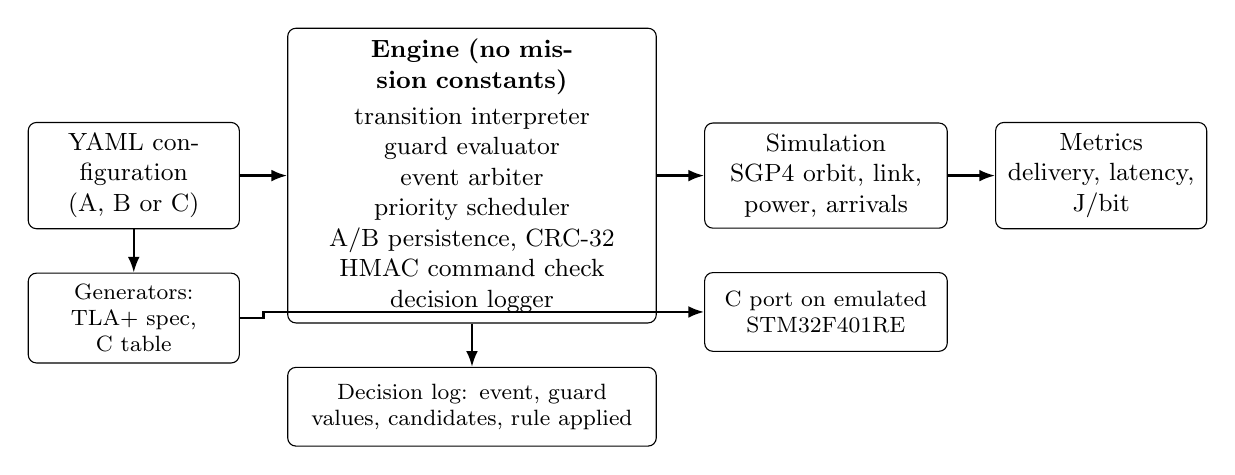
\begin{tikzpicture}[
  box/.style={draw, rounded corners=3pt, minimum height=1.0cm, align=center, font=\small, inner sep=4pt},
  arr/.style={-{Latex[length=2mm]}, thick}]
\node[box, text width=2.4cm] (cfg) {YAML configuration\\(A, B or C)};
\node[box, text width=4.4cm, right=0.6cm of cfg, minimum height=2.4cm] (engine)
  {\textbf{Engine (no mission constants)}\\[2pt] transition interpreter\\ guard evaluator\\ event arbiter\\ priority scheduler\\ A/B persistence, CRC-32\\ HMAC command check\\ decision logger};
\node[box, text width=2.8cm, right=0.6cm of engine] (sim) {Simulation\\SGP4 orbit, link,\\power, arrivals};
\node[box, text width=2.4cm, right=0.6cm of sim] (out) {Metrics\\delivery, latency,\\J/bit};
\node[box, text width=4.4cm, below=0.55cm of engine, font=\footnotesize] (log) {Decision log: event, guard values, candidates, rule applied};
\node[box, text width=2.4cm, below=0.55cm of cfg, font=\footnotesize] (gen) {Generators: TLA+ spec, C table};
\node[box, text width=2.8cm, below=0.55cm of sim, font=\footnotesize] (c) {C port on emulated STM32F401RE};
\draw[arr] (cfg) -- (engine); \draw[arr] (engine) -- (sim); \draw[arr] (sim) -- (out);
\draw[arr] (engine) -- (log); \draw[arr] (cfg) -- (gen); \draw[arr] (gen.east) -- ++(0.3,0) |- (c.west);
\end{tikzpicture}}
\caption{Framework architecture. The configuration file is the only mission-specific input; the TLA+ specification and the C transition table are generated from it.}
\label{fig:architecture}
\end{figure}

\subsection{Configuration schema}

A configuration has nine top-level keys: \code{meta}, \code{states}, \code{events}, \code{transitions}, \code{parameters}, \code{latches}, \code{data_class_priority}, \code{conflict_resolution} and \code{mode_exclusivity_groups}. A state has an identifier, name, documentation category, entry actions and an initial-state flag. An event has an identifier, a name and a source tag (\code{onboard}, \code{ground}, \code{scheduler} or \code{harness}). A transition has an identifier, a \code{from} list (or \code{"*"} for every state), an event, an optional guard, a target and a list of actions and requirement identifiers. The target is a state, \code{null} for a self-loop that only logs, or \code{reload_from_persistence}. Latches are declared once at top level with the transitions that set them and whether they survive a reset, so their semantics are not scattered across state entries.

\paragraph{Closed-world rule} A state--event pair with no matching transition, after expanding \code{"*"} and multi-state \code{from} lists and after evaluating guards, is illegal. The engine resolves it to a no-op: the state is unchanged, no action fires, and the decision log records the illegal pair. The rule belongs to the schema contract, so no configuration restates it.

\paragraph{Guards} Every guard in the three shipped configurations is a single binary comparison:
\begin{verbatim}
guard    ::= operand op operand
op       ::= "==" | "!=" | ">=" | "<=" | "<" | ">"
operand  ::= "context." ID | ID | PARAM_ID
           | "elapsed(" ID ")" | literal
PARAM_ID ::= /P[BC]?-\d{3}/
\end{verbatim}
\code{context.*} names refer to engine state that persists between steps and that only actions change. Bare identifiers such as \code{battery_soc} or \code{elevation} are telemetry supplied fresh on each step, which the engine reads but never writes. Boolean combinators are not implemented because no configuration needs them yet.

\paragraph{Actions} An action is either a context assignment (\code{set context.x = v}), which the engine applies, or an opaque identifier such as \code{enable_rf}, which the engine logs and does not execute. Wiring opaque actions to hardware is outside this software-only project; the decision log is the evidence that the correct action would have fired.

\subsection{Event conflict resolution and data-class priority}

Two orderings answer different questions and live under different keys. The data-class priority (\ttc{} $>$ SSTV $>$ Codec2/M17) is fixed by the mission's governance table and tells the scheduler which queued item to send next. The conflict-resolution ranking tells the arbiter which of several pending events to service first in one tick (Table~\ref{tab:conflict}). It is a configuration choice.

\begin{table}[t]
\centering
\small
\caption{Event conflict-resolution ranks shared by the three configurations.}
\label{tab:conflict}
\adjustbox{max width=\textwidth}{\begin{tabular}{@{}clp{0.48\textwidth}@{}}
\toprule
Rank & Category & Tie-break within the rank \\
\midrule
1 & Ground override, reset & Earliest timestamp; \code{RESET} wins ties against ground commands \\
2 & Fault, watchdog, power, comms loss & Timestamp, then event identifier \\
3 & Deployment lifecycle & Timestamp \\
4 & Scheduler, pass end & Data-class priority; \code{PASS_END} before any \code{SCHEDULER_SELECT_*} \\
5 & Routine & Timestamp \\
\bottomrule
\end{tabular}}
\end{table}

The arbiter sorts the pending events by rank, then by a data-class key within the scheduler rank (\code{PASS_END} before any select, selects in data-class priority order), then by timestamp, then with \code{RESET} ahead of other rank-1 events at an equal time, and finally by event identifier. The tie-break rule for each rank is read from the configuration's tie-break text, and text the arbiter does not recognise is a load error. It services the highest-ranked event that has a legal transition, drops higher-ranked events that have none, and keeps the rest queued with their original timestamps for the next tick. The step function itself still takes one event. The ranking matters for logging as well as for behaviour. When a ground safe-mode command and a natural pass end arrive in the same tick, the ground command is serviced, the pass end stays queued, and the log records a ground override with the queued event named.

An earlier version validated the ranks at load time but never consumed them: the simulation driver tried events in a fixed order, and in safe mode that order put autonomous recovery (rank~2) ahead of a ground exit (rank~1). Routing the driver through the arbiter left every seed-42 result, every evaluation-seed result and the recorded decision trace of Section~\ref{sec:cport} unchanged. It changed only the battery stress cases of Section~\ref{sec:stress}, where a recovery and a pass end can fall in the same tick.

\subsection{Persistence and decision log}

Each write goes to the inactive bank with sequence number $n+1$ and a fresh CRC-32. At boot both banks are validated and the valid bank with the higher sequence number is loaded. A reset during a write therefore leaves the previous bank intact, and the engine recovers the last consistent state. The guarantee assumes one fault at a time. If both banks are corrupt the engine boots from the initial state with an empty context and the deployment latch is lost. The sequence number that selects the newer bank lies outside the CRC, so a bit flip that raises the older bank's sequence number would load a stale but valid record. The C port's 32-bit sequence counter would wrap after $2^{32}$ saves, about 136 years at one save per second. Tests pin all three behaviours; none is fixed in this version. The decision log records every transition, including illegal-pair no-ops, with the triggering event and guard inputs, and every scheduler choice with the competing candidates and the rule that decided. The verification-matrix generator reads this log and the test results to map requirements to evidence.

\section{Reference configurations}\label{sec:configs}

\subsection{Config A: PocketQube reference}

\cfgA{} instantiates all three deployment mechanisms named in the use case: a separation switch, an RF-inhibit timer and an independent RF-beacon path. Both confirmation paths must agree before the one-way \code{deployment_confirmed} latch is set. The configuration has 10 states, 20 events and 24 transitions traced to 34 requirements (Fig.~\ref{fig:config-a}; the full table is in~\ref{app:trans-a}). The four downlink modes (\ttc{}, SSTV, voice, idle) are separate, mutually exclusive states.

\begin{figure}[t]
\centering
\resizebox{\textwidth}{!}{%
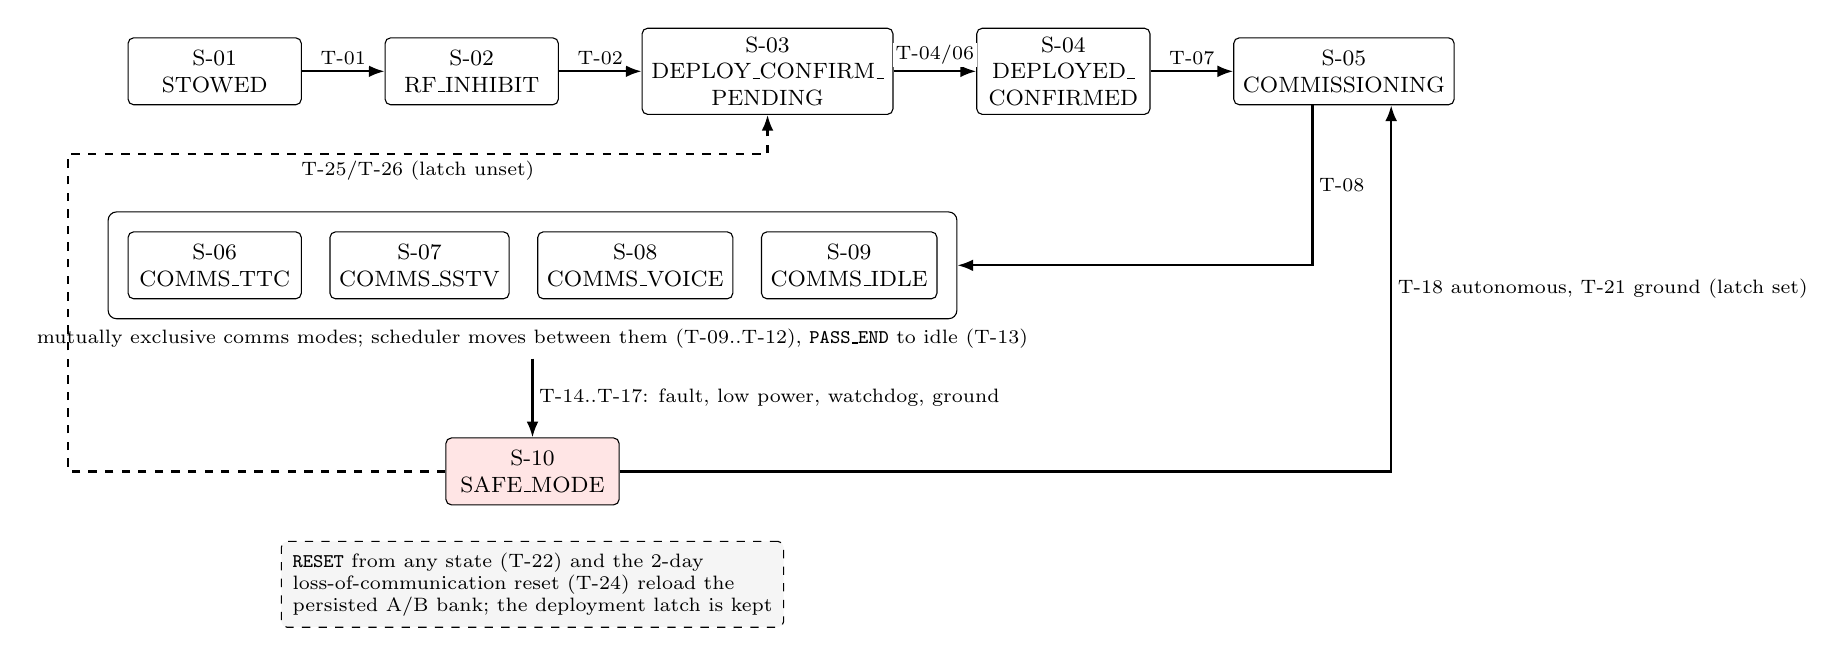
\begin{tikzpicture}[
  st/.style={draw, rounded corners=2pt, minimum height=0.85cm, minimum width=2.2cm, align=center, font=\footnotesize},
  saf/.style={st, fill=red!10},
  note/.style={draw, dashed, rounded corners=2pt, align=left, font=\scriptsize, fill=gray!8, inner sep=4pt},
  arr/.style={-{Latex[length=2mm]}, thick},
  lab/.style={font=\scriptsize, fill=white, inner sep=1pt}]
\node[st] (s1) {S-01\\STOWED};
\node[st, right=1.05cm of s1] (s2) {S-02\\RF\_INHIBIT};
\node[st, right=1.05cm of s2] (s3) {S-03\\DEPLOY\_CONFIRM\_\\PENDING};
\node[st, right=1.05cm of s3] (s4) {S-04\\DEPLOYED\_\\CONFIRMED};
\node[st, right=1.05cm of s4] (s5) {S-05\\COMMISSIONING};
\node[st, below=1.6cm of s1] (s6) {S-06\\COMMS\_TTC};
\node[st, right=0.35cm of s6] (s7) {S-07\\COMMS\_SSTV};
\node[st, right=0.35cm of s7] (s8) {S-08\\COMMS\_VOICE};
\node[st, right=0.35cm of s8] (s9) {S-09\\COMMS\_IDLE};
\begin{scope}[on background layer]
\node[draw, rounded corners=3pt, fit=(s6)(s9), inner sep=7pt, label={[font=\scriptsize]below:mutually exclusive comms modes; scheduler moves between them (T-09..T-12), \texttt{PASS\_END} to idle (T-13)}] (comms) {};
\end{scope}
\node[saf, below=1.5cm of comms] (s10) {S-10\\SAFE\_MODE};
\node[note, below=0.45cm of s10] (bank) {\texttt{RESET} from any state (T-22) and the 2-day\\loss-of-communication reset (T-24) reload the\\persisted A/B bank; the deployment latch is kept};
\draw[arr] (s1) -- node[lab, above=1pt]{T-01} (s2);
\draw[arr] (s2) -- node[lab, above=1pt]{T-02} (s3);
\draw[arr] (s3) -- node[lab, above=1pt]{T-04/06} (s4);
\draw[arr] (s4) -- node[lab, above=1pt]{T-07} (s5);
\draw[arr] ([xshift=-4mm]s5.south) |- node[lab, pos=0.25, right=1pt]{T-08} (comms.east);
\draw[arr] (s10.north -| comms.south) ++(0,1.0) -- node[lab, right=1pt]{T-14..T-17: fault, low power, watchdog, ground} (s10.north);
\draw[arr] (s10.east) -| node[lab, pos=0.75, right=1pt]{T-18 autonomous, T-21 ground (latch set)} ([xshift=6mm]s5.south);
\coordinate (lane) at ([xshift=-5mm]comms.west);
\coordinate (top) at ([yshift=-5mm]s3.south);
\draw[arr, dashed] (s10.west) -| (lane) |- node[lab, pos=0.75, below=1pt]{T-25/T-26 (latch unset)} (top) -- (s3.south);
\end{tikzpicture}}
\caption{Simplified \cfgA{} lifecycle. Safe-mode entries (T-14..T-17) also leave from COMMISSIONING and, for the ground command, from S-03 onward. Safe-mode exits return to commissioning only when the deployment latch is set and otherwise to S-03 (decision 0010). The full transition table is in~\ref{app:trans-a}.}
\label{fig:config-a}
\end{figure}

\cfgA{} lets the satellite leave safe mode on its own once recovery conditions hold (T-18), with a 15-percentage-point hysteresis between the 25\% entry and 40\% recovery charge thresholds to stop chattering. A ground operator can force or hold safe mode from S-03 onward (T-17) and can force an exit (T-21). Both exits are guarded on the deployment latch. A safe-mode episode entered from S-03 before confirmation returns to S-03 (T-25, T-26), keeping any confirmation path that had already asserted.

\subsection{Config B: single path, single mode}

\cfgB{} was written directly against the schema, before any engine existed, to test whether the schema could express a different mission without new fields. It differs from \cfgA{} on five axes (Table~\ref{tab:axes}): it confirms deployment from the switch and a debounce timer alone, has no RF-inhibit timer, has one downlink mode, and leaves safe mode only on a ground command. It has 7 states, 15 events, 15 transitions and 12 requirements. No schema change was needed: the schema has no minimum counts, a two-member mode-exclusivity group is legal, and removing autonomous recovery means leaving out the event and transition.

\subsection{Config C: the remaining axis combination}

\cfgA{} pairs dual-path deployment with autonomous recovery and \cfgB{} pairs single-path deployment with ground-only recovery. \cfgC{} adds single-path deployment with autonomous recovery: \cfgB{}'s seven-state structure plus an autonomous exit (T-16) next to the retained ground exit (T-12), for 16 transitions and 13 requirements. The simulation driver's recovery logic looks the recovery threshold up by parameter name, so it drove \cfgC{} without modification. \cfgC{} is synthetic. It is excluded from the policy comparison and uses the two-station scenario of Section~\ref{sec:groundstations} as its reference. The fourth combination, dual-path deployment with ground-only recovery, is not built.

\begin{table}[t]
\centering
\small
\caption{Structural differences between the three configurations.}
\label{tab:axes}
\adjustbox{max width=\textwidth}{\begin{tabular}{@{}lccc@{}}
\toprule
Axis & \cfgA{} & \cfgB{} & \cfgC{} \\
\midrule
Deployment confirmation & Switch+timer and beacon & Switch+debounce & Switch+debounce \\
RF-inhibit timer & 900~s & None & None \\
Downlink-mode states & 4 & 1 (+ idle) & 1 (+ idle) \\
Safe-mode exit & Autonomous or ground & Ground only & Autonomous or ground \\
States / events / transitions & 10 / 20 / 24 & 7 / 15 / 15 & 7 / 16 / 16 \\
Requirements & 34 & 12 & 13 \\
Parameters in YAML & 20 & 15 & 15 \\
\bottomrule
\end{tabular}}
\end{table}

\subsection{Defects found in design review}

A review held before the engine was written found five blocking defects. \cfgB{}'s deployment sequence deadlocked, because its only transition tested an elapsed-time guard on a timer that nothing started; the fix split it into an arm step and a check step, as \cfgA{} already did for its inhibit timer. The schema did not list \code{to: null} as legal although both configurations used it. One \cfgA{} event was missing from the conflict ranking, breaking the rule that every event appears in exactly one rank. The deployment-confirmation timeout parameters were declared but no guard read them, so a confirmation path that never asserted had no escalation; the fix extended the ground safe-mode transition to the deployment-pending states. The two parameters (P-011, P-012) are still read by no guard: a stalled confirmation is resolved only by a ground command, not by an on-board timeout, because leaving the pending state on a single unconfirmed signal would be unsupervised autonomy. Model checking later found that this fix had opened a path to commissioning without the latch (Section~\ref{sec:mc}). Finally, a ground-only safe-mode exit branch in \cfgA{} could never be reached. It was deleted, and \cfgB{} now carries that structural variant.

\subsection{Parameter governance}

Every numeric guard value not fixed by the use case is a parameter with a source and a confidence of \code{cited}, \code{assumed} or \code{tbd}, and every assumed value carries a written justification. The parameter register lists 21 \code{P-} parameters, of which 20 appear in the \cfgA{} YAML; the exception, P-021 (the A/B bank-swap policy), is an engine-level policy shared by all configurations. The register also lists 16 simulation constants; of the rows with a confidence tag, 16 are cited and 17 assumed. \cfgB{} and \cfgC{} use separate identifier namespaces (\code{PB-}, \code{PC-}) so that no reader assumes a value is shared. Table~\ref{tab:params} lists the \cfgA{} parameters that reach a guard or the simulation.

\begin{table}[t]
\centering
\footnotesize
\caption{\cfgA{} parameters that reach a guard or a simulation code path.}
\label{tab:params}
\begin{tabular}{@{}lp{0.37\textwidth}rp{0.29\textwidth}@{}}
\toprule
ID & Name & Value & Source (confidence) \\
\midrule
P-010 & \code{rf_inhibit_silence_timer_s} & 900 s & POQUITO~\cite{Franzese2026POQUITO} (cited) \\
P-013 & \code{battery_soc_safe_mode_entry_threshold_pct} & 25\% & Engineering judgement (assumed) \\
P-014 & \code{battery_soc_safe_mode_recovery_threshold_pct} & 40\% & 15-point hysteresis over P-013 (assumed) \\
P-015 & \code{link_quality_min_elevation_deg} & 10$^\circ$ & Ground-station practice (assumed) \\
P-016 & \code{fade_margin_db} & 3 dB & Engineering judgement (assumed) \\
P-017 & \code{watchdog_timeout_s} & 120 s & Masat-1 pattern~\cite{Latachi2020Masat} (assumed) \\
P-019 & \code{fault_count_threshold_for_latched_fault} & 3 & FDIR practice~\cite{Eshaq2025CubeSatFSW} (assumed) \\
P-023 & \code{ground_override_command_auth_model} & HMAC-SHA256 & Section~\ref{sec:auth} (assumed) \\
P-025 & \code{comms_loss_reset_timer_s} & 172,800 s & POQUITO~\cite{Franzese2026POQUITO} (cited) \\
\bottomrule
\end{tabular}
\end{table}

P-023 began as \code{tbd}: no defensible authentication model existed while authentication was out of scope, and the register said so. It became \code{assumed} when the work of Section~\ref{sec:auth} landed. The persistence policy was first drafted as a configuration parameter, but it belongs to the engine, so it is documented for its sources~\cite{Murphy2022NEPP,Chen2006EEPROM} and not exposed as per-mission data.

\section{Verification}\label{sec:verification}

\subsection{Test suite and fault injection}

For each configuration, the suite runs every transition row as a positive case and every state--event pair absent from the table as a no-op assertion. Every guarded row also has a guard-false case and a case at the threshold, with the inclusive or exclusive side taken from the requirement wording. Resets are injected at every transition boundary and, separately, at every byte boundary of a simulated non-volatile write, in the style of software-implemented fault injection~\cite{Hsueh1997FaultInjection}. A latch test checks that no sequence of resets or bank corruptions clears \code{deployment_confirmed} once set. A cross-configuration harness asserts three engine-level guarantees on every configuration: latch integrity (R-04, RB-02, RC-02), ground override from the RF-enabled states onward (R-22, RB-08, RC-08), and legality of \code{RESET} from every state with latch survival (R-27/R-29, RB-10, RC-10).

The suite grew from 539 tests at the verification freeze to \TestCount{} today, as later phases added the scheduler reordering hook, the published-orbit fixtures, \cfgC{}, the second ground station, authentication, the C port harnesses and, during review, the guard-boundary tests, the arbiter and the checks described below. All \TestCount{} tests pass. Statement coverage of the engine is 96.9\% and branch coverage 92.0\%. The verification matrix maps 34 \cfgA{}, 12 \cfgB{} and 13 \cfgC{} requirements to tests. It separates a requirement that a test merely names from one whose test result was recorded as an executed pass.

\subsection{Model checking}\label{sec:mc}

Tests enumerate cases chosen by people. To cover every reachable state, a generator writes a TLA+ module and TLC configuration from each YAML file on every run. The module tracks the control state, the latch, the Boolean context flags and the last durable snapshot of these. Every step either saves or leaves the previous snapshot in place, as a torn write would, and a reset restores the snapshot as the engine does. Guards that compare a Boolean context flag are encoded exactly. All other guards (timers, telemetry, parameters) are nondeterministic, which over-approximates the reachable behaviour.

TLC~\cite{Yu1999TLC} checks properties of two kinds. Generic ones come from the configuration: \code{TypeOK}, the persisted latch never clears, and once persisted the live latch is set. The others are written by hand from the requirements documents, naming states and events rather than reading them from the YAML: the latch rises only on the declared confirmation events (for \cfgA{}, only once both paths have confirmed); the RF-silent states are left only when the inhibit or debounce timer expires; safe mode is entered and left only through the declared events; ground safe-mode entry is available from exactly the RF-enabled states; reset is always available; and commissioning and every downlink state require the latch. Deadlock checking stays on.

The first run of this model found a defect in \cfgA{}. A ground safe-mode command from the confirmation-pending state, followed by either safe-mode exit, reached commissioning and then nominal downlink with the latch unset, in breach of the requirement that commissioning begins only after the latch is set. The engine reproduced the trace. It came from the design-review fix of Section~\ref{sec:configs}, which let T-17 start from the pending states while both exits still went to commissioning. Both exits are now guarded on the latch, and two new rows return an unlatched satellite to the pending state (decision 0010). After the fix all three configurations satisfy every property (Table~\ref{tab:tlc}). None of the simulation results moved, because the reference and stress runs enter safe mode only after deployment is confirmed.

The in-RAM form of the latch property is false in this model, and the checker script asserts that it stays false so that the persistence model cannot silently become vacuous: a reset that tears the save of the latch-setting step reloads the older bank. A version of this paper reported that the latch ``never clears'' from a model in which a reset returned to the initial state with the latch untouched. That model had no persistence, so the property held by construction. The model says nothing about timing, thresholds or liveness.

\begin{table}[t]
\centering
\small
\caption{TLC 2.19 results with the persistence model, after the \cfgA{} fix.}
\label{tab:tlc}
\adjustbox{max width=\textwidth}{\begin{tabular}{@{}lrrrrl@{}}
\toprule
Configuration & Declared states & States generated & Distinct states & Depth & Result \\
\midrule
\cfgA{}, before the fix & 10 & 41 & 16 & 4 & Latch-before-commissioning violated \\
\cfgA{} & 10 & 7,657 & 434 & 11 & No error \\
\cfgB{} & 7 & 1,798 & 121 & 9 & No error \\
\cfgC{} & 7 & 1,991 & 128 & 9 & No error \\
\bottomrule
\end{tabular}}
\end{table}

\subsection{Configuration mutation}

One YAML file feeds the engine, the TLA+ model and the C table, so a check derived from that file can share its errors. To measure this, 288 mutants of the three configurations were generated: dropped or retargeted transitions, toggled latch setters, swapped conflict ranks and changed guard operators. A mutant counts as killed if a check fails on it. TLC with only the configuration-derived properties killed the 18 that the loader already rejects and nothing else. With the hand-written properties it killed 77, about the same set as a breadth-first exploration of the real engine against the same requirements (73). The test suite as it stood before review killed 209, and all checks together killed 246, 96.1\% of the 256 non-equivalent mutants. Guard-operator mutants are killed almost entirely by the boundary tests, since TLC sees only the Boolean guards. Of the ten survivors, three are rank swaps (\cfgB{} ranks 2 and 3, \cfgC{} ranks 1 and 2 and ranks 2 and 3) that no test distinguishes, and seven remove ``must be able to'' behaviour, such as \cfgA{}'s watchdog entry into safe mode, that the hand-written properties do not yet state.

\section{Simulation environment}\label{sec:sim}

\subsection{Models}

The orbit is propagated with SGP4~\cite{Hoots1980STR3,Vallado2006SGP4} from POQUITO's published element set, the only one SatNOGS holds for the object (international designator 2025-009BY, epoch 2025-01-21 21:45:38.676~UTC, inclination 97.44$^\circ$, mean motion 15.172~rev/day, period 5,694.75~s). The simulation starts at the element-set epoch and is never propagated to the present date, because SGP4 error grows quickly away from epoch for a light, decaying object. The reference ground station is in Mumbai (19.076$^\circ$N, 72.878$^\circ$E). The link is an elevation-gated capacity model, not a link budget: the downlink runs at a constant 9600~bit/s whenever the maximum elevation over the ground stations is at least the P-015 mask. A margin model anchored at POQUITO's 10~dB at 15$^\circ$ with a slope of 0.5~dB per degree is reported for diagnostics, and a free-space path-loss check~\cite{Maral2009SatCom} supports the slope as a proxy. The gate never reads the margin, so the fade-margin parameter P-016 affects no reported number.

The power model assigns draw per transmit class: 0.0996~W idle and 3.415~W \ttc{} transmit (POQUITO figures), with SSTV and voice draws set to 1.5 and 1.25 times the \ttc{} draw because POQUITO carries neither payload. A simulation-side table maps each downlink state of each configuration to a fixed class (\cfgA{}'s three transmit states), to the class being served (the single \code{COMMS_ACTIVE} state of \cfgB{} and \cfgC{}), or to none (idle). The table is checked against the configuration's scheduler transitions at start-up. A downlink mode draws its class's transmit power for the first 156~s after the mode is entered, POQUITO's per-orbit beacon burst, and the idle draw afterwards (decision 0009). An earlier version looked the draw up by state name, which charged every \cfgB{} and \cfgC{} downlink at idle power; correcting it changed their energy and battery figures and no delivery or latency figure.

The battery is a lossless energy integrator. With tick $\Delta t = 10$~s, capacity $C = 4.5$~Wh and panel output $P_\mathrm{sol} = 0.4$~W when lit,
\begin{gather}
\mathrm{SoC}_k = \min\bigl(100,\ \max(0,\ \mathrm{SoC}_{k-1} + \Delta_k)\bigr), \\
\Delta_k = \frac{100\%}{C}\cdot\frac{\bigl(P_\mathrm{sol}\,\mathbb{1}_\mathrm{sun}(t_k) - P_\mathrm{draw}(t_k)\bigr)\Delta t}{3600~\mathrm{s\,h^{-1}}},
\end{gather}
starting from 100\%, where $P_\mathrm{draw}$ is the transmit draw of the current class inside the 156~s burst window and the idle draw otherwise, and $\mathbb{1}_\mathrm{sun}$ is a cylindrical-umbra test with no penumbra. There is no charge or discharge efficiency, voltage, temperature or ageing model, and surplus solar energy is discarded once the battery is full. The draw is taken from the state held before the tick's transitions, and the clamped state of charge is the telemetry the low-power and recovery guards read in the same tick. Over the 48~h reference window the satellite is in shadow 36.49\% of the time at the driver's 10~s tick.

Data items arrive as Poisson processes. \ttc{} arrives at 20 items per hour, from POQUITO's 3-minute beacon period~\cite{Franzese2024POQUITO4S}; SSTV and voice arrive at an illustrative 4 per hour. Sizes are uniform in 64--512~B (\ttc{}), 2,048--8,192~B (SSTV) and 256--1,536~B (voice), and deadlines are 300~s, 3,600~s and 900~s after arrival. Downlink runs at 9600~bit/s, and an item is served only if it fits in the remaining transmit time of the current tick.

Two delivery figures are reported. The \emph{window delivery ratio} is the fraction of generated items downlinked before the end of the 48~h run. The \emph{deadline success ratio} is the fraction delivered at or before their own deadline. ``Delivery'' without a qualifier means the first.

The baseline scheduler serves the highest-priority non-empty class whenever the link is up, earliest deadline first within a class. Because deadlines are a fixed offset from arrival for each class, this equals first-in first-out order except for an item that was held back and re-queued. The reference scenario is seed 42, 172,800~s (48~h) and a 10~s tick.

\subsection{Effect of adopting published mission data}

The first version of the simulation used a 10~Wh battery, 2.5~W of generation and a synthetic element set tuned to put the satellite almost overhead at epoch. With POQUITO's figures the first pass begins 8.31~h after epoch, only four passes above 10$^\circ$ occur in 48~h, and delivery falls from 99.9\% to 91.85\% (Table~\ref{tab:real-values}). Several test fixtures had assumed a pass near $t=0$ and were re-anchored to the computed pass times.

\begin{table}[t]
\centering
\small
\caption{Placeholder versus published POQUITO inputs for the reference scenario.}
\label{tab:real-values}
\adjustbox{max width=\textwidth}{\begin{tabular}{@{}lll@{}}
\toprule
Quantity & Placeholder & POQUITO-derived \\
\midrule
Battery capacity & 10.0 Wh & 4.5 Wh \\
Worst-case generation & 2.5 W & 0.4 W \\
Element set & Synthetic, tuned & Published, frozen at its epoch \\
Eclipse fraction (48 h) & 0\% & 36.5\% \\
Passes above 10$^\circ$ (48 h, Mumbai) & -- & 4 \\
Delivery success & 99.9\% & 91.85\% \\
\bottomrule
\end{tabular}}
\end{table}

\section{Results}\label{sec:results}

\subsection{Baseline}

Table~\ref{tab:baseline} gives the seed-42 baseline. \cfgA{} and \cfgB{} give the same figures on every metric. Delivery depends on link availability, throughput and arrivals, which the two configurations share; their structural differences sit in deployment and recovery, and neither configuration enters safe mode in this scenario. The state of charge never falls below 91.29\% with one station (70.65\% with two), so the safe-mode thresholds are exercised only by the stress cases of Section~\ref{sec:stress}.

\begin{table}[t]
\centering
\small
\caption{Baseline metrics, seed 42, 48 h, single Mumbai station (\cfgC{}: two stations).}
\label{tab:baseline}
\adjustbox{max width=\textwidth}{\begin{tabular}{@{}lrrr@{}}
\toprule
Metric & \cfgA{} & \cfgB{} & \cfgC{} \\
\midrule
Window delivery & 91.85\% & 91.85\% & 99.08\% \\
Deadline success & 2.61\% & 2.61\% & 18.14\% \\
\ttc{} latency, minimum (s) & 3.758 & 3.758 & 0.057 \\
\ttc{} latency, median (s) & 19,911.4 & 19,911.4 & 3,127.7 \\
\ttc{} latency, 95th percentile (s) & 39,819.9 & 39,819.9 & 18,824.6 \\
\ttc{} latency, maximum (s) & 42,723.4 & 42,723.4 & 23,731.6 \\
Energy per delivered bit (J/bit) & $3.389\times10^{-4}$ & $3.389\times10^{-4}$ & $4.703\times10^{-4}$ \\
\bottomrule
\end{tabular}}
\end{table}

Energy per delivered bit charges each item the draw in force while it was sent. An earlier write-up of this project reported $1.04\times10^{-5}$~J/bit for \cfgB{} and attributed the 33-fold difference to its simpler downlink design. That figure was idle power divided by bit rate, produced by the name-keyed power lookup described in Section~\ref{sec:sim}; with the per-class table, \cfgB{} matches \cfgA{} item for item.

The window figure hides a deadline problem (Table~\ref{tab:per-class}, Fig.~\ref{fig:per-class}). With a single station, 34 of 1,301 items (2.61\%) meet their deadline, and only 10 of 915 \ttc{} items reach the ground within 300~s; 836 arrive late and 69 are still queued at the end. Passes are short and hours apart, with the link up for 1.02\% of the run, so most items wait for the next pass. With the Svalbard station added (\cfgC{} reference), 236 items (18.14\%) meet their deadline, on-time \ttc{} delivery rises to 110 and undelivered \ttc{} items fall to 5. Contact time, not scheduling, is the binding constraint (Section~\ref{sec:policy}).

\begin{table}[t]
\centering
\small
\caption{Per-class outcomes, seed 42. Single station: \cfgA{} (\cfgB{} is identical). Two stations: \cfgC{}.}
\label{tab:per-class}
\begin{tabular}{@{}lrrrrrrr@{}}
\toprule
& & \multicolumn{3}{c}{One station} & \multicolumn{3}{c}{Two stations} \\
\cmidrule(lr){3-5}\cmidrule(l){6-8}
Class & Arrived & On time & Late & Never & On time & Late & Never \\
\midrule
\ttc{} & 915 & 10 & 836 & 69 & 110 & 800 & 5 \\
SSTV & 202 & 17 & 164 & 21 & 90 & 108 & 4 \\
Codec2/M17 & 184 & 7 & 161 & 16 & 36 & 145 & 3 \\
\bottomrule
\end{tabular}
\end{table}

\begin{figure}[t]
\centering
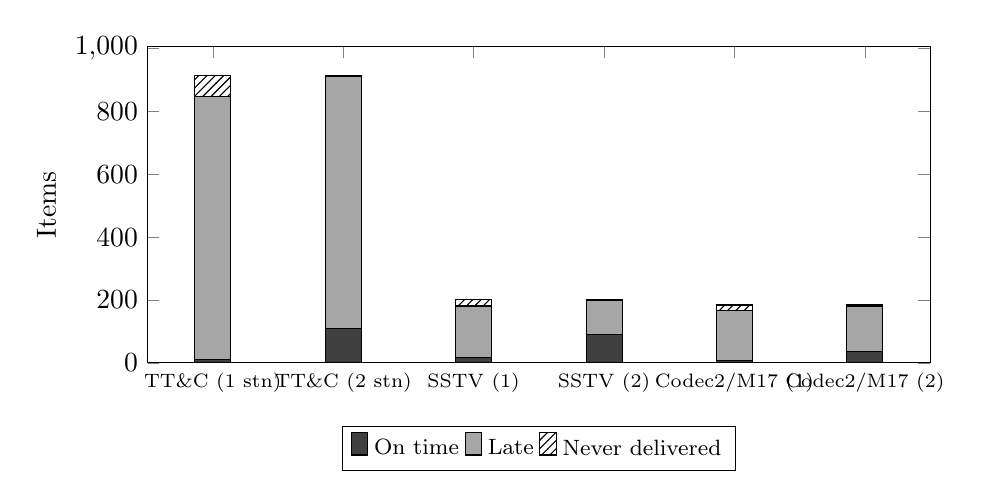
\begin{tikzpicture}
\begin{axis}[
  ybar stacked, bar width=13pt, width=0.95\textwidth, height=5.6cm,
  symbolic x coords={TTC-1,TTC-2,SSTV-1,SSTV-2,M17-1,M17-2},
  xticklabels={\ttc{} (1 stn), \ttc{} (2 stn), SSTV (1), SSTV (2), Codec2/M17 (1), Codec2/M17 (2)},
  xtick=data, x tick label style={font=\scriptsize}, ylabel={Items}, ymin=0,
  legend style={at={(0.5,-0.2)}, anchor=north, legend columns=3, font=\footnotesize}]
\addplot+[fill=black!75, draw=black] coordinates {(TTC-1,10) (TTC-2,110) (SSTV-1,17) (SSTV-2,90) (M17-1,7) (M17-2,36)};
\addplot+[fill=black!35, draw=black] coordinates {(TTC-1,836) (TTC-2,800) (SSTV-1,164) (SSTV-2,108) (M17-1,161) (M17-2,145)};
\addplot+[fill=white, draw=black, postaction={pattern=north east lines}] coordinates {(TTC-1,69) (TTC-2,5) (SSTV-1,21) (SSTV-2,4) (M17-1,16) (M17-2,3)};
\legend{On time, Late, Never delivered}
\end{axis}
\end{tikzpicture}
\caption{Delivery outcome per class over 48 h with one ground station (Mumbai) and two (Mumbai and Svalbard).}
\label{fig:per-class}
\end{figure}

\subsection{Multi-seed statistics}

Each baseline was repeated over 20 seeds and summarised by the mean and a normal-approximation 95\% confidence interval (Table~\ref{tab:multiseed}). The seed-42 delivery of 91.85\% lies inside the \cfgA{} interval of 91.61--92.45\%, a little below the 92.03\% mean, so the reference seed is representative and slightly pessimistic. \cfgC{} uses the two-station scenario.

\begin{table}[t]
\centering
\small
\caption{Twenty-seed means with 95\% confidence intervals.}
\label{tab:multiseed}
\adjustbox{max width=\textwidth}{\begin{tabular}{@{}lllll@{}}
\toprule
Config & Window delivery & Deadline success & \ttc{} p95 latency (s) & Energy/bit ($10^{-4}$ J/bit) \\
\midrule
A & 0.9203 [0.9161, 0.9245] & 0.0253 [0.0238, 0.0269] & 39,845.8 [39,633.9, 40,057.8] & 3.744 [3.653, 3.835] \\
B & 0.9203 [0.9161, 0.9245] & 0.0253 [0.0238, 0.0269] & 39,845.8 [39,633.9, 40,057.8] & 3.744 [3.653, 3.835] \\
C & 0.9933 [0.9921, 0.9946] & 0.1705 [0.1663, 0.1747] & 19,411.2 [19,162.8, 19,659.7] & 4.814 [4.790, 4.838] \\
\bottomrule
\end{tabular}}
\end{table}

\subsection{Learned policy versus rule-based baseline}\label{sec:policy}

Four policies are compared, all of which decide only whether to serve the head of the queue now or hold it. Two baselines always serve: one orders items within a class by earliest deadline (EDF)~\cite{Liu1973EDF}, the scheduler's default, and one by queue insertion (FIFO). Every other policy also uses EDF ordering. The one-step lookahead policy rolls the full simulation (orbit, power, engine and scheduler) forward 900~s (90 ticks) under each choice, follows an always-serve EDF policy after the first tick, and picks the choice with fewer \ttc{} deadline misses, then fewer other misses, then less energy. It is a heuristic, not a bound: it looks one decision ahead and treats a deadline beyond its horizon as met. An earlier version of this paper called it an oracle and an upper bound, which was wrong. The decision tree is a binary tree with Gini splits, a maximum depth of 4 and at least five samples per leaf, trained on the lookahead policy's state--action pairs~\cite{Quinlan1986ID3,Hussein2017Imitation}. One tree is trained per scenario on seeds 1000--1019 and every policy is evaluated on the disjoint seeds 6000--6019. Arrivals depend only on the seed, so the policies are compared on paired runs, with percentile-bootstrap confidence intervals (10,000 resamples) over the 20 evaluation seeds.

To show how much room any policy has, an offline clairvoyant relaxation is solved for each seed. It knows every arrival and every link-up tick, keeps only the per-tick link budget, allows an item to be split across ticks, and ignores power, safe mode, the state machine and the class priority. Every schedule the simulator can produce is feasible in it, so no policy can exceed it. The window-delivery bound is solved exactly by the Moore--Hodgson rule on the time-reversed problem and the deadline bound is a fluid upper bound.

\begin{table}[t]
\centering
\small
\caption{Policy comparison, \cfgA{}, reference scenario, mean over evaluation seeds 6000--6019 with 95\% bootstrap intervals.}
\label{tab:policy}
\adjustbox{max width=\textwidth}{\begin{tabular}{@{}lllll@{}}
\toprule
Policy & Window delivery & Deadline success & Energy/bit ($10^{-4}$ J/bit) & Energy drawn (Wh) \\
\midrule
Baseline, FIFO & 92.08\% [91.69, 92.42] & 2.81\% [2.63, 2.99] & 3.636 [3.539, 3.736] & 6.362 [6.315, 6.408] \\
Baseline, EDF & 92.08\% [91.69, 92.42] & 2.77\% [2.58, 2.96] & 3.641 [3.558, 3.729] & 6.382 [6.340, 6.424] \\
Lookahead & 92.08\% [91.69, 92.42] & 2.66\% [2.49, 2.83] & 2.774 [2.660, 2.889] & 6.099 [6.068, 6.130] \\
Tree & 92.08\% [91.69, 92.42] & 2.77\% [2.58, 2.96] & 3.641 [3.558, 3.729] & 6.382 [6.340, 6.424] \\
Clairvoyant bound & 92.20\% & 3.09\% & -- & -- \\
\bottomrule
\end{tabular}}
\end{table}

Window delivery is identical for all four policies on every evaluation seed, in the reference, worst-case and two-station scenarios and on both \cfgA{} and \cfgB{} (Table~\ref{tab:policy}); the only exception is a FIFO--EDF ordering effect of 0.09 points in the worst case. All policies come within 0.12 points of the bound. At seed 42 every policy delivers 1,195 of 1,301 items, which is the bound exactly: each undelivered item arrives after the last pass of the run. No policy can meet more than about 3.1\% of deadlines with one mid-latitude station.

The tree learns to serve almost everywhere, holding at most 3 times in about 25,000 decisions, and so reproduces the EDF baseline. RQ3 therefore has a negative answer: the learned policy does not beat the rule-based one. The lookahead policy holds at about 3\% of decision points on \cfgA{}. Against the EDF baseline it lowers energy per delivered bit by 24\% (paired difference $-8.7\times10^{-5}$~J/bit, 95\% CI $[-10.2, -7.1]\times10^{-5}$, lower on 20 of 20 seeds) and the total energy drawn by 4.4\% ($-0.28$~Wh $[-0.33, -0.23]$). The saving is real in battery terms but smaller than the per-bit figure suggests; holding avoids some mode switches and therefore some 156~s transmit bursts, though the mechanism was not isolated further. It costs 0.11 points of deadline success $[-0.14, -0.08]$ and 5.2~s of \ttc{} p95 latency $[1.4, 10.0]$. On \cfgB{} the lookahead policy's per-bit saving is only 2\% (14 of 20 seeds lower). Within-class ordering matters little: EDF minus FIFO is at most 0.1 points on any metric.

Requirement R-20 asks that the policies be analysable for cost on the same inputs. Table~\ref{tab:complexity} gives the asymptotic cost of one decision and host timings on the same 50 decision contexts, spread over the seed-42 run, with 500 samples per policy.

\begin{table}[t]
\centering
\small
\caption{Cost of one \texttt{decide()} call, \cfgA{}, host CPython.}
\label{tab:complexity}
\begin{tabular}{@{}llrr@{}}
\toprule
Policy & Asymptotic cost & Median & p95 \\
\midrule
Baseline & $O(1)$ & 0.02~\textmu s & 0.02~\textmu s \\
Tree & $O(d)$, $d=4$ & 0.48~\textmu s & 0.51~\textmu s \\
Lookahead & $O(2h)$, $h=90$ ticks & 8.51~ms & 10.02~ms \\
\bottomrule
\end{tabular}
\end{table}

All three are constant per decision in the asymptotic sense, but the lookahead policy runs a full orbit, power, engine and scheduler rollout per tick and costs about 18,000 times the tree. The tree was not run on the microcontroller. It needs at most four floating-point comparisons, which by instruction count should take well under 1~\textmu s at 84~MHz; this is an estimate, not a measurement.

\subsection{Parameter sensitivity}

A one-at-a-time sweep varied each assumed \cfgA{} parameter that reaches a guard or the simulation, holding the others at their shipped values. Parameters that no code path reads (P-011, P-012, P-016, P-017, P-018, P-020, P-022, P-024) were excluded after a repository-wide search. The fade margin P-016 is among them because the link gate ignores the margin.

\begin{table}[t]
\centering
\small
\caption{One-at-a-time sensitivity, \cfgA{}, seed 42.}
\label{tab:sensitivity}
\begin{tabular}{@{}llrr@{}}
\toprule
Parameter & Value & Delivery & Energy/bit (J/bit) \\
\midrule
P-013 safe-mode entry SoC & 15 / 25 / 35\% & 91.85\% (all) & $3.389\times10^{-4}$ (all) \\
P-014 recovery SoC & 30 / 40 / 50\% & 91.85\% (all) & $3.389\times10^{-4}$ (all) \\
\multirow{3}{*}{P-015 elevation mask} & 5$^\circ$ & 91.93\% & $3.896\times10^{-4}$ \\
 & 10$^\circ$ (baseline) & 91.85\% & $3.389\times10^{-4}$ \\
 & 15$^\circ$ & 80.63\% & $3.502\times10^{-4}$ \\
P-019 fault threshold & 1 / 3 / 5 & 91.85\% (all) & $3.389\times10^{-4}$ (all) \\
\bottomrule
\end{tabular}
\end{table}

Only the elevation mask moves the metrics (Table~\ref{tab:sensitivity}, Fig.~\ref{fig:sens}). Raising it from 10$^\circ$ to 15$^\circ$ costs 11.2 percentage points of delivery, while lowering it to 5$^\circ$ gains 0.08 points and raises energy per bit by 15\%. The charge thresholds have no effect because the battery never falls to them in the 48~h window. The fault threshold has none because the reference scenario injects no faults; the fault path is exercised by the engine tests and by stress case ST-3.

\begin{figure}[t]
\centering
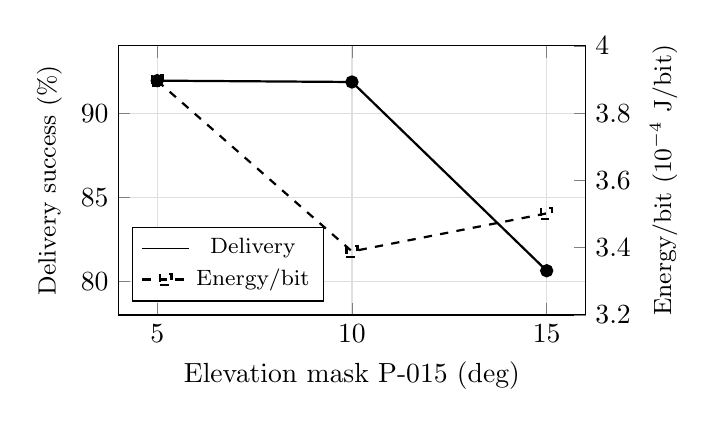
\begin{tikzpicture}
\begin{axis}[
  width=0.62\textwidth, height=5.0cm, xlabel={Elevation mask P-015 (deg)}, ylabel={Delivery success (\%)},
  xtick={5,10,15}, ymin=78, ymax=94, grid=major, grid style={gray!25},
  axis y line*=left, ylabel style={font=\small}]
\addplot[thick, mark=*] coordinates {(5,91.93) (10,91.85) (15,80.63)}; \label{pl:del}
\end{axis}
\begin{axis}[
  width=0.62\textwidth, height=5.0cm, xtick=\empty, axis y line*=right, axis x line=none,
  ylabel={Energy/bit ($10^{-4}$ J/bit)}, ymin=3.2, ymax=4.0, ylabel style={font=\small},
  legend style={at={(0.03,0.05)}, anchor=south west, font=\footnotesize}]
\addlegendimage{/pgfplots/refstyle=pl:del}\addlegendentry{Delivery}
\addplot[thick, dashed, mark=square] coordinates {(5,3.896) (10,3.389) (15,3.502)}; \addlegendentry{Energy/bit}
\end{axis}
\end{tikzpicture}
\caption{Effect of the elevation mask on delivery and energy per delivered bit (\cfgA{}, seed 42).}
\label{fig:sens}
\end{figure}

The SSTV and voice draws are scaled placeholders, so their per-class energy was computed over a $\pm30\%$ band on the scaling ratio. SSTV ranges from $2.236\times10^{-4}$ to $4.116\times10^{-4}$~J/bit (ratio 1.05--1.95) and Codec2/M17 from $3.113\times10^{-4}$ to $5.781\times10^{-4}$~J/bit (ratio 0.875--1.625). These bands are the uncertainty on those classes until a measured payload draw is available.

\subsection{Compounding worst case}

A one-at-a-time sweep cannot show interactions. A second scenario sets every parameter to its adverse end at once (entry 35\%, recovery 50\%, mask 15$^\circ$, fault threshold 1) and raises the arrival rates to 80 \ttc{} items per hour (four times nominal) and 40 SSTV and 40 voice items per hour (ten times nominal). Delivery falls from 91.85\% to 47.34\% on all three configurations, a drop of 44.51 points, and deadline success from 2.61\% to 0.37\%, while \ttc{} p95 latency rises from 39,819.9~s to 40,089.5~s. Energy per bit changes little, falling to $3.274\times10^{-4}$~J/bit. The clairvoyant bound of Section~\ref{sec:policy} for this scenario is 59.1\% at seed 42; it ignores the power and safe-mode losses that the adverse thresholds cause, so the gap is an upper limit on what a better policy could recover. The 91.85\% headline therefore describes a nominal load, and an overloaded single-station mission with a strict mask delivers under half its data.

\subsection{Battery and fault stress cases}\label{sec:stress}

The reference scenario never comes near the safe-mode thresholds, so three stress cases exercise them, each changing one simulation input and no configuration value. ST-1 starts at 25.2\% charge at the element-set epoch, which is in eclipse. ST-2 uses an aged 1.5~Wh battery and both stations. ST-3 injects a fault at each configuration's latched-fault threshold for 1,800~s from 8.35~h, inside the first pass (Table~\ref{tab:stress}).

\begin{table}[t]
\centering
\small
\caption{Battery and fault stress cases, seed 42.}
\label{tab:stress}
\adjustbox{max width=\textwidth}{\begin{tabular}{@{}llrrrrrr@{}}
\toprule
Config & Case & Safe entries & First exit (h) & Time in safe (s) & Min SoC & Window delivery & Deadline success \\
\midrule
\multirow{3}{*}{A} & ST-1 & 1 & 3.96 & 14,250 & 24.72\% & 91.85\% & 2.61\% \\
 & ST-2 & 76 & 22.28 & 27,730 & 15.20\% & 99.08\% & 18.14\% \\
 & ST-3 & 1 & 8.85 & 1,800 & 91.30\% & 88.16\% & 1.31\% \\
\midrule
\multirow{3}{*}{B} & ST-1 & 1 & 8.31 & 29,610 & 24.92\% & 91.85\% & 2.61\% \\
 & ST-2 & 28 & 22.28 & 29,390 & 23.98\% & 99.08\% & 18.14\% \\
 & ST-3 & 1 & 20.36 & 43,220 & 91.30\% & 88.16\% & 1.31\% \\
\midrule
\multirow{3}{*}{C} & ST-1 & 1 & 2.41 & 8,340 & 24.92\% & 91.85\% & 2.61\% \\
 & ST-2 & 28 & 22.28 & 4,090 & 23.98\% & 99.08\% & 18.14\% \\
 & ST-3 & 1 & 8.85 & 1,800 & 91.30\% & 88.16\% & 1.31\% \\
\bottomrule
\end{tabular}}
\end{table}

ST-1 separates the three recovery models. \cfgA{} leaves safe mode on its own at 40\% charge after 3.96~h and \cfgC{} at 35\% after 2.41~h, while ground-only \cfgB{} waits for the first pass at 8.31~h. Recovery comes before that pass in every case, so delivery is unaffected. In ST-3, \cfgA{} and \cfgC{} resume as soon as the fault clears, while \cfgB{} misses the rest of the pass and stays in safe mode for 12~h until the next one; all three lose part of the first pass. ST-2 shows a limitation of the simulated ground segment rather than of the state machines. The ground-operator model releases safe mode at any tick inside a pass, whatever the charge, so when the battery crosses the entry threshold during a pass the next transmit burst sends it straight back, and safe mode cycles 76 times on \cfgA{} and 28 times on \cfgB{} and \cfgC{}. Under that model, safe mode does not protect the battery during passes. A release rule that waits for the recovery threshold would remove the cycling but has not been adopted.

\subsection{Second ground station}\label{sec:groundstations}

The orbit and driver accept a list of stations, taking the maximum elevation over the list each tick; with the default single station every earlier result is reproduced exactly. Adding Svalbard (78.23$^\circ$N, 15.39$^\circ$E), a high-latitude site that sees a sun-synchronous orbit on most revolutions, raises link-up time from 1,760~s to 10,160~s in 48~h (1.02\% to 5.88\% of the run, +477.3\%) and delivery from 91.85\% to 99.08\% (Table~\ref{tab:gs}). Svalbard was chosen to measure the effect of geometry; it makes no claim about POQUITO's own ground segment, and the reference scenario keeps the single Mumbai station. Deadline success rises from 2.61\% to 18.14\% and energy per bit to $4.703\times10^{-4}$~J/bit. Results for \cfgA{} and \cfgB{} are identical, since station coverage is independent of the lifecycle structure in which they differ.

\begin{table}[t]
\centering
\small
\caption{Effect of a second ground station, seed 42 (\cfgA{} and \cfgB{} identical).}
\label{tab:gs}
\adjustbox{max width=\textwidth}{\begin{tabular}{@{}lrrrrr@{}}
\toprule
Stations & Link-up time (s) & Share of run & Window delivery & Deadline success & \ttc{} p95 (s) \\
\midrule
Mumbai & 1,760 & 1.02\% & 91.85\% & 2.61\% & 39,819.9 \\
Mumbai + Svalbard & 10,160 & 5.88\% & 99.08\% & 18.14\% & 18,824.6 \\
\bottomrule
\end{tabular}}
\end{table}

\section{Ground-command authentication}\label{sec:auth}

Every event carried a source tag from the start, but a review found that nothing read it: a ground-sourced event such as \code{GROUND_OVERRIDE_EXIT_SAFE} fired exactly like an on-board one. The engine now signs and verifies ground commands with HMAC-SHA256~\cite{RFC2104,Bellare1996HMAC,NIST2015SHS} from the Python standard library, comparing signatures in constant time. The signed message is the event identifier joined to the simulated timestamp, so a captured signature cannot be replayed for another event or another time.

Authentication has three modes. With no secret, the engine runs as an unauthenticated simulation: the source tag is not read and every older call site behaves as before. Every experiment in this paper uses this mode. With \code{require_auth}, a missing or empty secret is a configuration error that stops the engine before any transition is evaluated, so a misconfigured engine cannot silently accept unsigned commands, and a missing, forged or wrong-key signature on a ground-sourced event makes that event illegal whatever its guard would have said. With \code{replay_protection}, each ground command also carries a counter that is signed with the event and timestamp. A command whose counter is not greater than the last accepted one is rejected, which stops the same message being accepted twice at the same time, and a verified counter is consumed even if the command's guard then fails, so a rejected command cannot be replayed later when the guard would pass. The counter is stored in the persisted context and survives a reset that reloads a valid record. It does not survive a cold start with no valid record; earlier commands then become acceptable again, and a test pins that limit. Unit tests cover each mode, including tampered and non-integer counters and an on-board event being unaffected.

The C port verifies the two-field message without the counter. When built with authentication enabled it rejects every ground command until a secret is provisioned; replay protection is implemented in the Python engine only. The model stops at the software layer. Key provisioning and rotation, link-layer protection as in CCSDS SDLS~\cite{CCSDS2022SDLS}, and a freshness window in place of the exact timestamp are out of scope. The exact-timestamp match works here only because the driver signs and dispatches within one tick. Falco's principles~\cite{Falco2019SpaceCyber} list what a flight implementation would still need.

\section{C port and emulated-hardware equivalence}\label{sec:cport}

\subsection{Scope and toolchain}

Earlier versions of this work stated that no on-device verification had been attempted because no hardware was available. To narrow that gap, the decision logic was ported to C and run on a Renode~\cite{Renode} emulation of a Nucleo-F401RE (STM32F401RE, Cortex-M4) under Zephyr~\cite{Zephyr}. The claim is limited to this: the C decision logic produces the same decisions as the Python engine on an emulated Cortex-M4. It says nothing about power, real-time behaviour, cycle timing or RF. The Python engine and simulation were not modified for the port, which lives in a separate directory.

Renode ships no description for this board, so the platform reuses Renode's STM32F4 SoC description, the same one its STM32F407 Discovery board uses. The two parts share the register map for the peripherals used here (GPIO, USART2, NVIC, RCC). Toolchain versions are pinned: Zephyr 4.2.2, Zephyr SDK 0.17.4 (arm-zephyr-eabi GCC 12.2.0) and West 1.5.0. The original runs used Renode 1.16.1 and the revision runs 1.17.0.

The port covers the fixed-array priority queue, the guard evaluator, the step function, A/B persistence and HMAC-SHA256 through mbedTLS. A script generates the transition table from the YAML file. The C signing routine handles only whole-second, non-negative timestamps below $10^{15}$, which covers every call site in the repository (the driver's tick loop and the 53 hand-written transition fixtures, all of which use integer times), and it returns false outside that range. A golden-vector test against the Python signer shows no mismatch. Host and firmware exchange newline-terminated ASCII lines over USART2 (\code{INJECT} and test-hook commands in, \code{DECISION}, \code{OK} and \code{ERROR} out). Test hooks are compiled out by default, and the protocol is test plumbing only. The default engine image uses 35,668~B of flash (6.8\% of 512~KB) and 11,648~B of RAM (11.9\% of 96~KB), most of the RAM being the 8~KB interrupt stack; the generated configuration table is 6.3~KB of the code.

The event-ordering function of the arbiter is also ported, with its rank and tie-break keys generated from the configuration. A host harness compares it with the Python arbiter on every single event, every ordered pair of events at equal and different times, and 2,000 random pending sets per configuration: 7,711 cases across the three configurations, with no mismatch. Flipping the \code{RESET} tie-break in the C code produced 59 mismatches, so the comparison detects that kind of error. The bridge still injects one event per line, so the firmware image does not yet call the arbiter.

\subsection{Full-run equivalence}

The replay captures every call the simulation driver makes to the engine's step function during the seed-42, 48~h, 10~s \cfgA{} run. It does this by temporarily replacing the driver's imported name with a recorder that calls through to the real function, so neither the engine nor the driver changes. Exploratory calls made by the bootstrap's breadth-first path search are excluded, because their results are never applied to the running state. The captured inputs are then fed to the firmware over one continuous Renode session, and each response is compared with the Python result for the same call.

\begin{table}[t]
\centering
\small
\caption{\cfgA{} equivalence run: C firmware on emulated STM32F401RE versus Python engine.}
\label{tab:cport}
\begin{tabular}{@{}lr@{}}
\toprule
Quantity & Value \\
\midrule
Step calls captured & 35,763 \\
\quad legal & 18,306 \\
\quad illegal (no-op) & 17,457 \\
Simulated ticks & 17,281 \\
Mismatches & 0 \\
Repeat run & Byte-identical logs \\
\bottomrule
\end{tabular}
\end{table}

All 35,763 decisions matched (Table~\ref{tab:cport}). Most illegal calls are \code{POWER_LOW} and \code{PASS_END} attempted on nearly every tick once the satellite is in a comms state. That is the closed-world no-op of Section~\ref{sec:design}, now shown to agree between the two implementations. \cfgB{} and \cfgC{} were not run end to end.

\subsection{Contact-window gate for ground commands}

Command injection over two emulated nodes, satellite and ground station, was also considered. Renode's STM32F4 description has no radio peripheral, so its wireless medium cannot be used. A second node on a UART hub would have needed either its own orbital code, which the project rules forbid re-deriving, or a relay that only echoes host decisions. The first breaks the project rules and the second adds no ground logic of its own, so neither was built.

The host bridge already stands in for the ground segment, so it gained a contact-window gate instead. The gate computes contact windows with the simulation's own pass finder for \cfgC{}'s two-station scenario and refuses to write an \code{INJECT} line unless the simulated time is inside a window, signing the command with the engine's HMAC routine when a secret is configured. Four cases on \cfgC{}'s T-14 (\code{UPLINK_CMD_GENERIC}, a ground event) passed in one Renode session, twice. A gated command outside a window was refused and no bytes reached the UART. A follow-up read timed out, confirming that nothing was sent. The same command at the same time with the gate bypassed was accepted by the firmware, which shows the block is ground-side policy. A gated command inside a window (345~s, within the window from 160 to 530~s at 26.91$^\circ$ peak elevation) went through with a valid signature. Authentication on board and pass timing on the ground are separate concerns: a satellite accepts an authentic command without knowing whether it is over a station.

\section{Re-running and revising the reported results}\label{sec:rerun}

Every experiment was re-run against the committed sources on 6 and 7 October 2026 and compared with the committed results. That re-run reproduced the simulation, policy and model-checking numbers of the time. A review of the resulting manuscript then raised points that led to the code changes described in the preceding sections, and every experiment was regenerated from the revised sources on 14 October 2026 (Table~\ref{tab:rerun}).

\begin{table}[t]
\centering
\footnotesize
\caption{Outcome of the revision run on 14 October 2026, against the numbers of the earlier version.}
\label{tab:rerun}
\begin{tabular}{@{}p{0.30\textwidth}p{0.62\textwidth}@{}}
\toprule
Experiment & Outcome \\
\midrule
Test suite & \TestCount{} tests, all passed \\
Baseline, A/B/C, 1 and 20 seeds & Delivery and latency unchanged; \cfgB{} and \cfgC{} energy corrected; deadline success added \\
Policy comparison & Reworked: four policies, held-out seeds, bootstrap intervals, clairvoyant bound \\
Sensitivity and power uncertainty & Unchanged \\
Two-station analysis & Unchanged except \cfgB{} energy; deadline success added \\
Compounding worst case & Unchanged except \cfgB{} energy; stress cases added \\
Policy timing & Re-measured on identical inputs (Table~\ref{tab:complexity}) \\
TLC & New persistence model; \cfgC{} added; \cfgA{} defect found and fixed \\
C-port equivalence & \ReplayOutcome \\
\bottomrule
\end{tabular}
\end{table}

The review and re-runs found the following defects in the earlier version, each corrected above. The power model's name-keyed lookup charged \cfgB{} and \cfgC{} downlinks at idle power; the earlier version had noticed the anomaly but described it rather than fixing it. The policy called an oracle and an upper bound was a one-step heuristic, and on deadline success it does worse than always serving. The model behind ``the deployment latch never clears'' had no persistence, so the property was close to vacuous; the stronger model found the \cfgA{} commissioning defect. The conflict ranks the paper described as governing event order were validated but never read at run time. Authentication without a secret silently accepted unsigned ground commands, and the same signed message could be accepted twice at the same time. Delivery was reported only within the run window, which hides how few items meet their deadline.

Two tests compile the C authentication module against the host's mbedTLS. The host library had moved to mbedTLS 4.2, which declares \code{mbedtls_md_hmac} only when \code{MBEDTLS_DECLARE_PRIVATE_IDENTIFIERS} is set; the host test build now defines it. The firmware builds against the mbedTLS bundled with Zephyr and is unaffected.

The October re-run stated that the Zephyr SDK was not installed, so the firmware was not rebuilt. That was wrong: a pinned SDK was present in a working copy on the same machine. For the revision the firmware was rebuilt from the current sources, including the two new \cfgA{} transitions, and the full reference trace was replayed over Renode on the rebuilt image in one continuous session: all 35,763 calls matched, and both the Python trace and the firmware decision log were byte-identical to the archived ones. The revised engine produces a Python trace identical, call for call, to the archived one: the new transitions start in safe mode, which the reference run never enters. Reading the C-port records also showed that the flash and RAM figures quoted in an earlier draft (15,988~B and 4,544~B) belong to the first echo-loop firmware used to prove the toolchain, not to the engine firmware; and that the timestamp restriction of Section~\ref{sec:cport} rests on 53 hand-written fixtures, not the ``about 150'' a design record states. Finally, the eclipse fraction quoted earlier, 36.46\%, was sampled every 60~s; the driver's 10~s tick gives 36.49\%.

\section{Discussion}\label{sec:discussion}

\paragraph{RQ1, generality} One engine runs the three configurations unchanged, and the schema took no new fields for \cfgB{} or \cfgC{}. The three guarantees most tied to the engine (latch integrity, ground override, reset legality) hold on all three under one harness. The \cfgC{} recovery path ran on simulation code written before \cfgC{} existed, because that code looks parameters up by name. The generality has limits. All three configurations use one latch, the same five conflict categories and single-comparison guards. A mission that needs compound guards or nested states would need schema work.

\paragraph{RQ2, resets} \code{RESET} is legal from every state on every configuration, and a reset during a write never leaves a corrupted state loaded. Once the deployment latch has been durably saved, it survives every reset and any single-bank corruption; TLC confirms this over every reachable state of all three configurations, and the tests add the byte-level write interruptions that the model does not represent. Two cases lose the latch: a reset that tears the save of the step that set it, which leaves the satellite to confirm deployment again, and corruption of both banks. Checking hand-written requirements rather than properties read from the configuration is what found the \cfgA{} commissioning defect; checks derived from the same file as the engine caught none of the mutants that the loader accepted.

\paragraph{RQ3, learned policy} The tie is a property of the scenario. The clairvoyant bound shows that every policy already delivers almost everything that the contact windows allow, so no scheduling policy can raise window delivery by more than a fraction of a point. Passes are rare and short, so whatever is queued when the link comes up should go out. The room that remains is in energy: the lookahead policy draws 4.4\% less at a small cost in deadline success, and the tree did not capture that behaviour at depth 4. A learned policy would have more room in a scenario where holding pays, for example with a battery near its safe-mode threshold during a pass.

\paragraph{RQ4, port} The C decision logic matched every decision of a full 48~h run. This is evidence that the logic survives the move from a dynamically typed language to fixed-size C structures on a Cortex-M4 instruction set. Timing and power behaviour on silicon remain untested.

\paragraph{What the numbers say about the mission} The single-station deadline performance is poor: 2.61\% of items and about 1\% of \ttc{} items meet their deadline, against a bound of about 3\% for any policy. That follows from orbit geometry: four passes in 48~h over Mumbai. A scheduler cannot fix it, but a second station raises deadline success to 18\%. The elevation mask is the parameter to pin down first, since it is the only assumed value that moves delivery.

\section{Limitations and threats to validity}\label{sec:limitations}

The ground-operator model is one fixed assumption: a ground override is issued at any tick inside a pass after safe-mode entry, whatever the charge, which causes the cycling of stress case ST-2. The reference scenario injects no faults and never approaches the safe-mode thresholds; only the stress cases and the engine tests exercise those paths, and no watchdog event is simulated. SSTV and voice draws, data-arrival rates for those classes, sizes and deadlines are illustrative. The battery model is lossless with flat solar input, and the link is gated on elevation alone at a constant rate, so the fade margin has no effect. The orbit is a single element set frozen at its epoch, and the results describe that 48~h window only.

Model checking encodes only the Boolean guards; timers, thresholds and parameter values are nondeterministic, and liveness is not checked, so threshold errors are caught by the boundary tests and not by TLC. The persistence guarantee assumes one corrupted bank at a time, the bank sequence number is outside the CRC, and the C port's sequence counter can in principle wrap. The deployment-confirmation timeouts are documentation only; a stalled confirmation needs a ground command. The C port has been checked end to end on \cfgA{} only, on emulated hardware, and its arbiter is checked on the host but not called by the firmware. Physical deployment, power measurement, flight qualification, RF implementation, deployer mechanics and on-board anomaly detection are outside the project. Opaque actions such as \code{enable_rf} are only logged; RF state is implied by the state-machine state. Authentication excludes key management and link-layer security, and replay protection exists in the Python engine only.

\section{Adopting the framework for a new mission}\label{sec:migration}

A new mission supplies data only. It writes a configuration file under the schema: its own states, events and transitions; parameters with sources; latches that must survive resets; its downlink priority; a conflict ranking; and mode-exclusivity groups. It then works through the parameter register and replaces each assumed value with a cited one from its ICD as the ICD matures. The TLA+ specification and the C transition table are regenerated from the new file, and the cross-configuration harness and model checker run against it unchanged. The hand-written requirement properties are not generated; the mission writes them from its own requirements, and that independence is what lets them catch errors in the configuration. The elevation mask, the charge thresholds and the payload transmit draws are the first values to replace, in that order, given the sensitivity results.

\section{Conclusion}\label{sec:conclusion}

A table-driven engine with no mission constants ran three structurally different PocketQube lifecycles unchanged. Once durably saved, its deployment latch survived every reset tested and every state TLC reached, after model checking against hand-written requirements found and closed a path to commissioning without the latch. The decision logic reproduced every one of 35,763 decisions when ported to C on an emulated Cortex-M4. Driven by POQUITO's published orbit and power figures, the rule-based scheduler delivered 91.85\% of items within 48~h from one station, the most any policy could deliver for that seed, but only 2.61\% by their deadlines; a second station raised these to 99.08\% and 18.14\%. A learned policy did not improve on the rule-based one, and the elevation mask was the only assumed parameter that changed delivery. Re-running the experiments and responding to review corrected a power-model defect, a mislabelled policy, a near-vacuous model-checking result and an unimplemented ordering claim, all recorded in Section~\ref{sec:rerun}.

\section*{Data and code availability}
Configuration files, engine, simulation, generators, TLA+ specifications, firmware sources and the archived equivalence logs are in the project repository, \url{https://github.com/inikunjrathi/pocketqube-fsm}. Every table in Sections~\ref{sec:verification}--\ref{sec:rerun} is produced by a named generator under \code{tools/} or by the scripts in \code{mcu/host_bridge/}; the commands are listed in \code{report/elsevier/README.md}. The reference orbit is POQUITO's element set (NORAD 98706), hard-coded in \code{sim/scenario.py}, whose two element lines, each newline-terminated, have the SHA-256 digest \code{69c5aec63c09c5652c2d8a76a09f647f} \code{615a04d8370d41f61aca6c23439ff581}; it is propagated with the \code{sgp4} Python package, version 2.27.

\section*{Declaration of competing interest}
The author declares no competing financial interests or personal relationships that could have influenced the work reported in this paper.

\section*{Funding}
This research received no specific grant from any funding agency in the public, commercial or not-for-profit sectors.

\section*{CRediT authorship contribution statement}
\textbf{Nikunj Rathi:} Conceptualization, Methodology, Software, Validation, Formal analysis, Investigation, Writing -- original draft, Writing -- review \& editing.

\appendix
\section{Transition tables}\label{app:transitions}
% Generated by make_transition_tables.py. Do not hand-edit.
\Needspace{12\baselineskip}
\subsection{Config A (24 transitions)}\label{app:trans-a}
{\scriptsize
\begin{longtable}{@{}p{0.05\textwidth}p{0.11\textwidth}p{0.25\textwidth}p{0.25\textwidth}p{0.06\textwidth}p{0.10\textwidth}@{}}
\caption{Config A transition table, generated from \texttt{config/config-a.yaml}.}\\
\toprule
ID & From & Event & Guard & To & Req. \\
\midrule
\endfirsthead
\toprule
ID & From & Event & Guard & To & Req. \\
\midrule
\endhead
T-01 & S-01 & SEPARATION\_\allowbreak DETECTED & -- & S-02 & \mbox{R-01} \\
T-02 & S-02 & RF\_\allowbreak INHIBIT\_\allowbreak TIMER\_\allowbreak EXPIRED & \texttt{elapsed(rf\_\allowbreak inhibit\_\allowbreak timer) $\geq$ P-010} & S-03 & \mbox{R-02} \\
T-03 & S-03 & DEPLOY\_\allowbreak CONFIRM\_\allowbreak PATH\_\allowbreak A & \texttt{context.path\_\allowbreak b\_\allowbreak confirmed == false} & S-03 & \mbox{R-03}, \mbox{R-07} \\
T-04 & S-03 & DEPLOY\_\allowbreak CONFIRM\_\allowbreak PATH\_\allowbreak A & \texttt{context.path\_\allowbreak b\_\allowbreak confirmed == true} & S-04 & \mbox{R-03}, \mbox{R-04}, \mbox{R-07} \\
T-05 & S-03 & DEPLOY\_\allowbreak CONFIRM\_\allowbreak PATH\_\allowbreak B & \texttt{context.path\_\allowbreak a\_\allowbreak confirmed == false} & S-03 & \mbox{R-03}, \mbox{R-07} \\
T-06 & S-03 & DEPLOY\_\allowbreak CONFIRM\_\allowbreak PATH\_\allowbreak B & \texttt{context.path\_\allowbreak a\_\allowbreak confirmed == true} & S-04 & \mbox{R-03}, \mbox{R-04}, \mbox{R-07} \\
T-07 & S-04 & ENTER\_\allowbreak COMMISSIONING & -- & S-05 & \mbox{R-05} \\
T-08 & S-05 & COMMISSIONING\_\allowbreak COMPLETE & -- & S-06 & \mbox{R-06} \\
T-09 & S-06..S-09 & SCHEDULER\_\allowbreak SELECT\_\allowbreak TTC & -- & S-06 & \mbox{R-11}, \mbox{R-13}, \mbox{R-17} \\
T-10 & S-06..S-09 & SCHEDULER\_\allowbreak SELECT\_\allowbreak SSTV & -- & S-07 & \mbox{R-11}, \mbox{R-13} \\
T-11 & S-06..S-09 & SCHEDULER\_\allowbreak SELECT\_\allowbreak VOICE & -- & S-08 & \mbox{R-11}, \mbox{R-13} \\
T-12 & S-06..S-09 & SCHEDULER\_\allowbreak SELECT\_\allowbreak IDLE & -- & S-09 & \mbox{R-11}, \mbox{R-13}, \mbox{R-18} \\
T-13 & S-06..S-09 & PASS\_\allowbreak END & \texttt{elevation $<$ P-015} & S-09 & \mbox{R-12} \\
T-14 & S-05..S-09 & FAULT\_\allowbreak DETECTED & \texttt{fault\_\allowbreak count $\geq$ P-019} & S-10 & \mbox{R-21}, \mbox{R-31} \\
T-15 & S-05..S-09 & POWER\_\allowbreak LOW & \texttt{battery\_\allowbreak soc $\leq$ P-013} & S-10 & \mbox{R-21}, \mbox{R-25}, \mbox{R-31} \\
T-16 & S-05..S-09 & WATCHDOG\_\allowbreak TIMEOUT & -- & S-10 & \mbox{R-21}, \mbox{R-31} \\
T-17 & S-03..S-10 & GROUND\_\allowbreak SAFE\_\allowbreak MODE\_\allowbreak CMD & -- & S-10 & \mbox{R-22}, \mbox{R-31} \\
T-18 & S-10 & AUTONOMOUS\_\allowbreak RECOVERY\_\allowbreak CONDITIONS\_\allowbreak MET & \texttt{context.deployment\_\allowbreak confirmed == true} & S-05 & \mbox{R-05}, \mbox{R-23}, \mbox{R-25}, \mbox{R-31} \\
T-21 & S-10 & GROUND\_\allowbreak OVERRIDE\_\allowbreak EXIT\_\allowbreak SAFE & \texttt{context.deployment\_\allowbreak confirmed == true} & S-05 & \mbox{R-05}, \mbox{R-24}, \mbox{R-31} \\
T-25 & S-10 & AUTONOMOUS\_\allowbreak RECOVERY\_\allowbreak CONDITIONS\_\allowbreak MET & \texttt{context.deployment\_\allowbreak confirmed == false} & S-03 & \mbox{R-05}, \mbox{R-23}, \mbox{R-31} \\
T-26 & S-10 & GROUND\_\allowbreak OVERRIDE\_\allowbreak EXIT\_\allowbreak SAFE & \texttt{context.deployment\_\allowbreak confirmed == false} & S-03 & \mbox{R-05}, \mbox{R-24}, \mbox{R-31} \\
T-22 & any & RESET & -- & reload & \mbox{R-04}, \mbox{R-27}, \mbox{R-28}, \mbox{R-29} \\
T-23 & any & UPLINK\_\allowbreak CMD\_\allowbreak GENERIC & -- & (self) & \mbox{R-31}, \mbox{R-33} \\
T-24 & S-03..S-10 & COMMS\_\allowbreak LOSS\_\allowbreak TIMEOUT & \texttt{elapsed(ground\_\allowbreak contact\_\allowbreak timer) $\geq$ P-025} & reload & \mbox{R-34} \\
\bottomrule
\end{longtable}}

\Needspace{12\baselineskip}
\subsection{Config B (15 transitions)}\label{app:trans-b}
{\scriptsize
\begin{longtable}{@{}p{0.05\textwidth}p{0.11\textwidth}p{0.25\textwidth}p{0.25\textwidth}p{0.06\textwidth}p{0.10\textwidth}@{}}
\caption{Config B transition table, generated from \texttt{config/config-b.yaml}.}\\
\toprule
ID & From & Event & Guard & To & Req. \\
\midrule
\endfirsthead
\toprule
ID & From & Event & Guard & To & Req. \\
\midrule
\endhead
T-01 & S-01 & SEPARATION\_\allowbreak DETECTED & -- & S-02 & \mbox{RB-01} \\
T-02 & S-02 & SWITCH\_\allowbreak DEBOUNCE\_\allowbreak ELAPSED & \texttt{elapsed(switch\_\allowbreak debounce\_\allowbreak timer) $\geq$ PB-002} & S-03 & \mbox{RB-01}, \mbox{RB-02} \\
T-03 & S-03 & ENTER\_\allowbreak COMMISSIONING & -- & S-04 & \mbox{RB-03} \\
T-04 & S-04 & COMMISSIONING\_\allowbreak COMPLETE & -- & S-05 & \mbox{RB-04} \\
T-05 & S-05, S-06 & SCHEDULER\_\allowbreak SELECT\_\allowbreak ACTIVE & -- & S-05 & \mbox{RB-05} \\
T-06 & S-05, S-06 & SCHEDULER\_\allowbreak SELECT\_\allowbreak IDLE & -- & S-06 & \mbox{RB-05} \\
T-07 & S-05, S-06 & PASS\_\allowbreak END & \texttt{elevation $<$ PB-006} & S-06 & \mbox{RB-06} \\
T-08 & S-04..S-06 & FAULT\_\allowbreak DETECTED & \texttt{fault\_\allowbreak count $\geq$ PB-005} & S-07 & \mbox{RB-07}, \mbox{RB-11} \\
T-09 & S-04..S-06 & POWER\_\allowbreak LOW & \texttt{battery\_\allowbreak soc $\leq$ PB-003} & S-07 & \mbox{RB-07}, \mbox{RB-11} \\
T-10 & S-04..S-06 & WATCHDOG\_\allowbreak TIMEOUT & -- & S-07 & \mbox{RB-07}, \mbox{RB-11} \\
T-11 & S-03..S-07 & GROUND\_\allowbreak SAFE\_\allowbreak MODE\_\allowbreak CMD & -- & S-07 & \mbox{RB-08}, \mbox{RB-11} \\
T-12 & S-07 & GROUND\_\allowbreak OVERRIDE\_\allowbreak EXIT\_\allowbreak SAFE & -- & S-04 & \mbox{RB-09}, \mbox{RB-11} \\
T-13 & any & RESET & -- & reload & \mbox{RB-02}, \mbox{RB-10} \\
T-14 & any & UPLINK\_\allowbreak CMD\_\allowbreak GENERIC & -- & (self) & \mbox{RB-11} \\
T-15 & S-03..S-06 & COMMS\_\allowbreak LOSS\_\allowbreak TIMEOUT & \texttt{elapsed(ground\_\allowbreak contact\_\allowbreak timer) $\geq$ PB-011} & reload & \mbox{RB-12} \\
\bottomrule
\end{longtable}}

\Needspace{12\baselineskip}
\subsection{Config C (16 transitions)}\label{app:trans-c}
{\scriptsize
\begin{longtable}{@{}p{0.05\textwidth}p{0.11\textwidth}p{0.25\textwidth}p{0.25\textwidth}p{0.06\textwidth}p{0.10\textwidth}@{}}
\caption{Config C transition table, generated from \texttt{config/config-c.yaml}.}\\
\toprule
ID & From & Event & Guard & To & Req. \\
\midrule
\endfirsthead
\toprule
ID & From & Event & Guard & To & Req. \\
\midrule
\endhead
T-01 & S-01 & SEPARATION\_\allowbreak DETECTED & -- & S-02 & \mbox{RC-01} \\
T-02 & S-02 & SWITCH\_\allowbreak DEBOUNCE\_\allowbreak ELAPSED & \texttt{elapsed(switch\_\allowbreak debounce\_\allowbreak timer) $\geq$ PC-002} & S-03 & \mbox{RC-01}, \mbox{RC-02} \\
T-03 & S-03 & ENTER\_\allowbreak COMMISSIONING & -- & S-04 & \mbox{RC-03} \\
T-04 & S-04 & COMMISSIONING\_\allowbreak COMPLETE & -- & S-05 & \mbox{RC-04} \\
T-05 & S-05, S-06 & SCHEDULER\_\allowbreak SELECT\_\allowbreak ACTIVE & -- & S-05 & \mbox{RC-05} \\
T-06 & S-05, S-06 & SCHEDULER\_\allowbreak SELECT\_\allowbreak IDLE & -- & S-06 & \mbox{RC-05} \\
T-07 & S-05, S-06 & PASS\_\allowbreak END & \texttt{elevation $<$ PC-006} & S-06 & \mbox{RC-06} \\
T-08 & S-04..S-06 & FAULT\_\allowbreak DETECTED & \texttt{fault\_\allowbreak count $\geq$ PC-005} & S-07 & \mbox{RC-07}, \mbox{RC-11} \\
T-09 & S-04..S-06 & POWER\_\allowbreak LOW & \texttt{battery\_\allowbreak soc $\leq$ PC-003} & S-07 & \mbox{RC-07}, \mbox{RC-11} \\
T-10 & S-04..S-06 & WATCHDOG\_\allowbreak TIMEOUT & -- & S-07 & \mbox{RC-07}, \mbox{RC-11} \\
T-11 & S-03..S-07 & GROUND\_\allowbreak SAFE\_\allowbreak MODE\_\allowbreak CMD & -- & S-07 & \mbox{RC-08}, \mbox{RC-11} \\
T-12 & S-07 & GROUND\_\allowbreak OVERRIDE\_\allowbreak EXIT\_\allowbreak SAFE & -- & S-04 & \mbox{RC-09}, \mbox{RC-11} \\
T-13 & any & RESET & -- & reload & \mbox{RC-02}, \mbox{RC-10} \\
T-14 & any & UPLINK\_\allowbreak CMD\_\allowbreak GENERIC & -- & (self) & \mbox{RC-11} \\
T-15 & S-03..S-06 & COMMS\_\allowbreak LOSS\_\allowbreak TIMEOUT & \texttt{elapsed(ground\_\allowbreak contact\_\allowbreak timer) $\geq$ PC-011} & reload & \mbox{RC-12} \\
T-16 & S-07 & AUTONOMOUS\_\allowbreak RECOVERY\_\allowbreak CONDITIONS\_\allowbreak MET & \texttt{battery\_\allowbreak soc $\geq$ PC-012} & S-04 & \mbox{RC-13} \\
\bottomrule
\end{longtable}}


\bibliographystyle{elsarticle-num}
\bibliography{refs}

\end{document}
